\documentclass[10pt,letterpaper]{article}
\usepackage[utf8]{inputenc}
\usepackage{amsmath}
\usepackage{amsfonts}
\usepackage{amssymb}
\usepackage{graphicx}

\author{Brock Ellefson}
\title{ANTY101 Lab 2}
\begin{document}
\maketitle
\newpage


%%%%%%%%%%%%%%%%%%%%%%%%%%%%%%%%%%%%%%%%%%%%%%%%%%%%%%%%%%%%%
\begin{figure}[]
	\centering
		\begin{minipage}[b]{0.4\textwidth}
			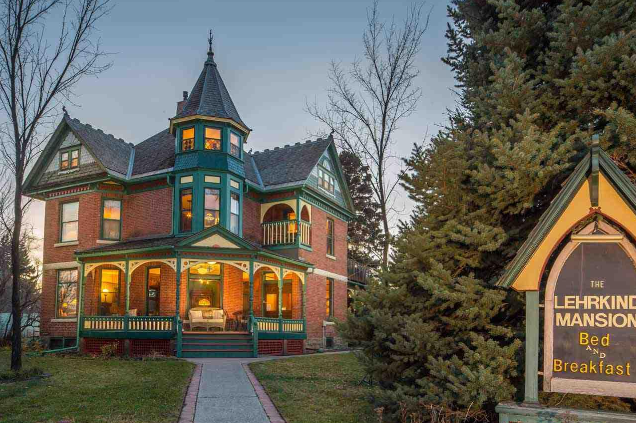
\includegraphics[width=\textwidth]{house1pic1.png}
    		\caption{719 N Wallace Avenue}
  		\end{minipage}
  \hfill
  		\begin{minipage}[b]{0.4\textwidth}
    		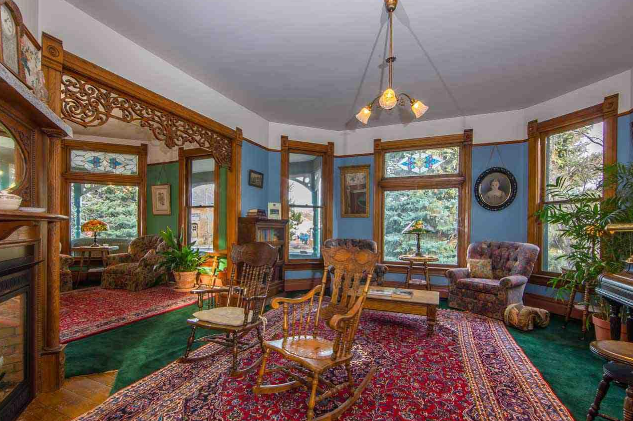
\includegraphics[width=\textwidth]{house1pic2.png}
    		\caption{719 N Wallace Avenue}
  		\end{minipage}
\end{figure}

	
The Lehrkind Mansion Bed and Breakfast is an iconic Queen Anne style building of Bozeman that was constructed in 1897. The exterior is made mainly of brick. However there is green wood trim outlining the house. 3 floors, 11 bedrooms. There is also a separate guest house on the tail end of the BnB, complete with a full bathroom and 3 bedrooms, totaling to 4,626 square feet. The driveway is paved with fine gravel. The entrance has a beautiful open porch.
%%%%%%%%%%%%%%%%%%%%%%%%%%%%%%%%%%%%%%%%%%%%%%%%%%%%%%%%%%%%%

\begin{figure}[h]
	\centering
		\begin{minipage}[b]{0.4\textwidth}
			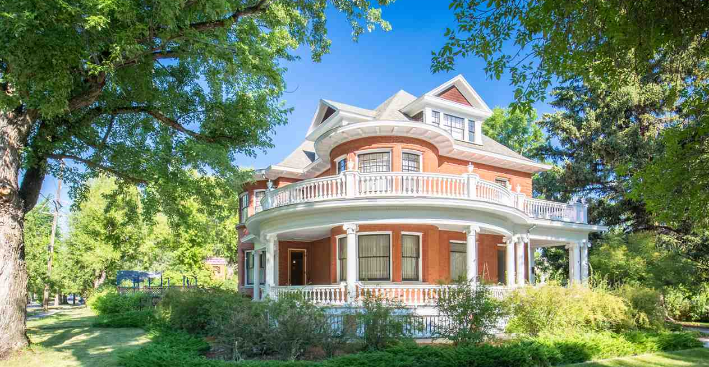
\includegraphics[width=\textwidth]{house2pic1.png}
    		\caption{725 S Willson Avenue}
  		\end{minipage}
  \hfill
  		\begin{minipage}[b]{0.4\textwidth}
    		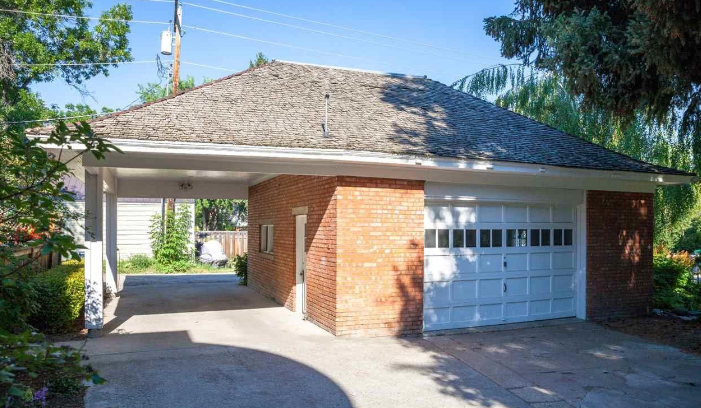
\includegraphics[width=\textwidth]{house2pic2.png}
    		\caption{725 S Willson Avenue}
  		\end{minipage}
\end{figure}

Next is one of the most iconic mansions in the historical district of Bozeman. This Queen Anne/Colonial Revival styled mansion was built in 1906. At first glance, the things about that catch your eye will by its curved-pane, oversized windows in the front, its brick modeling, and large veranda. The woodwork is used with a beautiful tiger oak that really pops. The roof is solid asphalt. On the inside, there are hardwood floors, vaulted ceilings, walk-in closets, and a gas powered fireplace on the west side. Over the 3 floors, there are four bedrooms, two full bathrooms, one half bathroom, and a  remodeled kitchen, along with a patio, porch, and balcony. All of this totals to a whopping 5915 square feet. There are beautiful shrubs and bushes surrounding the perimeter of the house.
%%%%%%%%%%%%%%%%%%%%%%%%%%%%%%%%%%%%%%%%%%%%%%%%%%%%%%%%%%%%%
\newpage 
%%%%%%%%%%%%%%%%%%%%%%%%%%%%%%%%%%%%%%%%%%%%%%%%%%%%%%%%%%%%%

\begin{figure}
	\centering
		\begin{minipage}[b]{0.4\textwidth}
			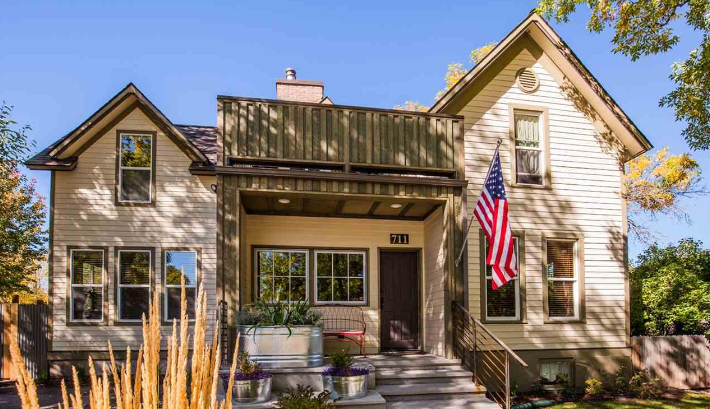
\includegraphics[width=\textwidth]{house3pic1.png}
    		\caption{711 N Black}
  		\end{minipage}
  \hfill
  		\begin{minipage}[b]{0.4\textwidth}
    		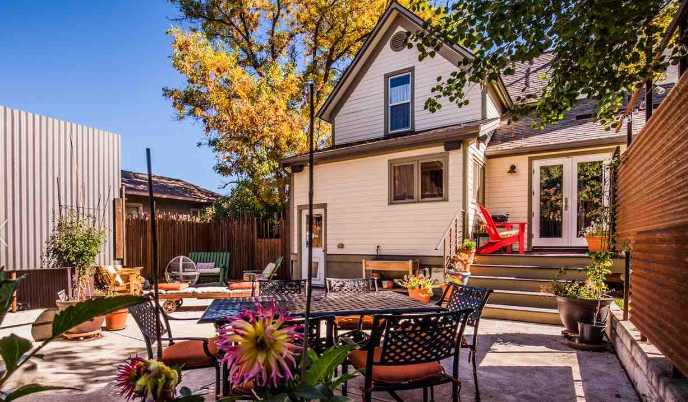
\includegraphics[width=\textwidth]{house3pic2.png}
    		\caption{711 N Black}
  		\end{minipage}
\end{figure}

Even though this house was remodeled once in 2008 and again in 2014 it still captures the very elegant traditional 1900 architectural style. Complete with a total of 7 bedrooms and 7 bathrooms, this mansion can hold quite a large family. Most of the interior decorated with a hardwood or tile floor. There is a fireplace and a beautiful patio, complemented with an equally gorgeous deck and porch. The roof is made mostly of asphalt, however there are some shingles as well. All of these totaling about 2,890 square feet, making it the smallest building I analyzed. However this building does have a paved driveway, a detached garage, and even a greenhouse. So despite not being as large as the other buildings, it still has great value
%%%%%%%%%%%%%%%%%%%%%%%%%%%%%%%%%%%%%%%%%%%%%%%%%%%%%%%%%%%%%

\begin{figure}[h]
	\centering
		\begin{minipage}[b]{0.25\textwidth}
			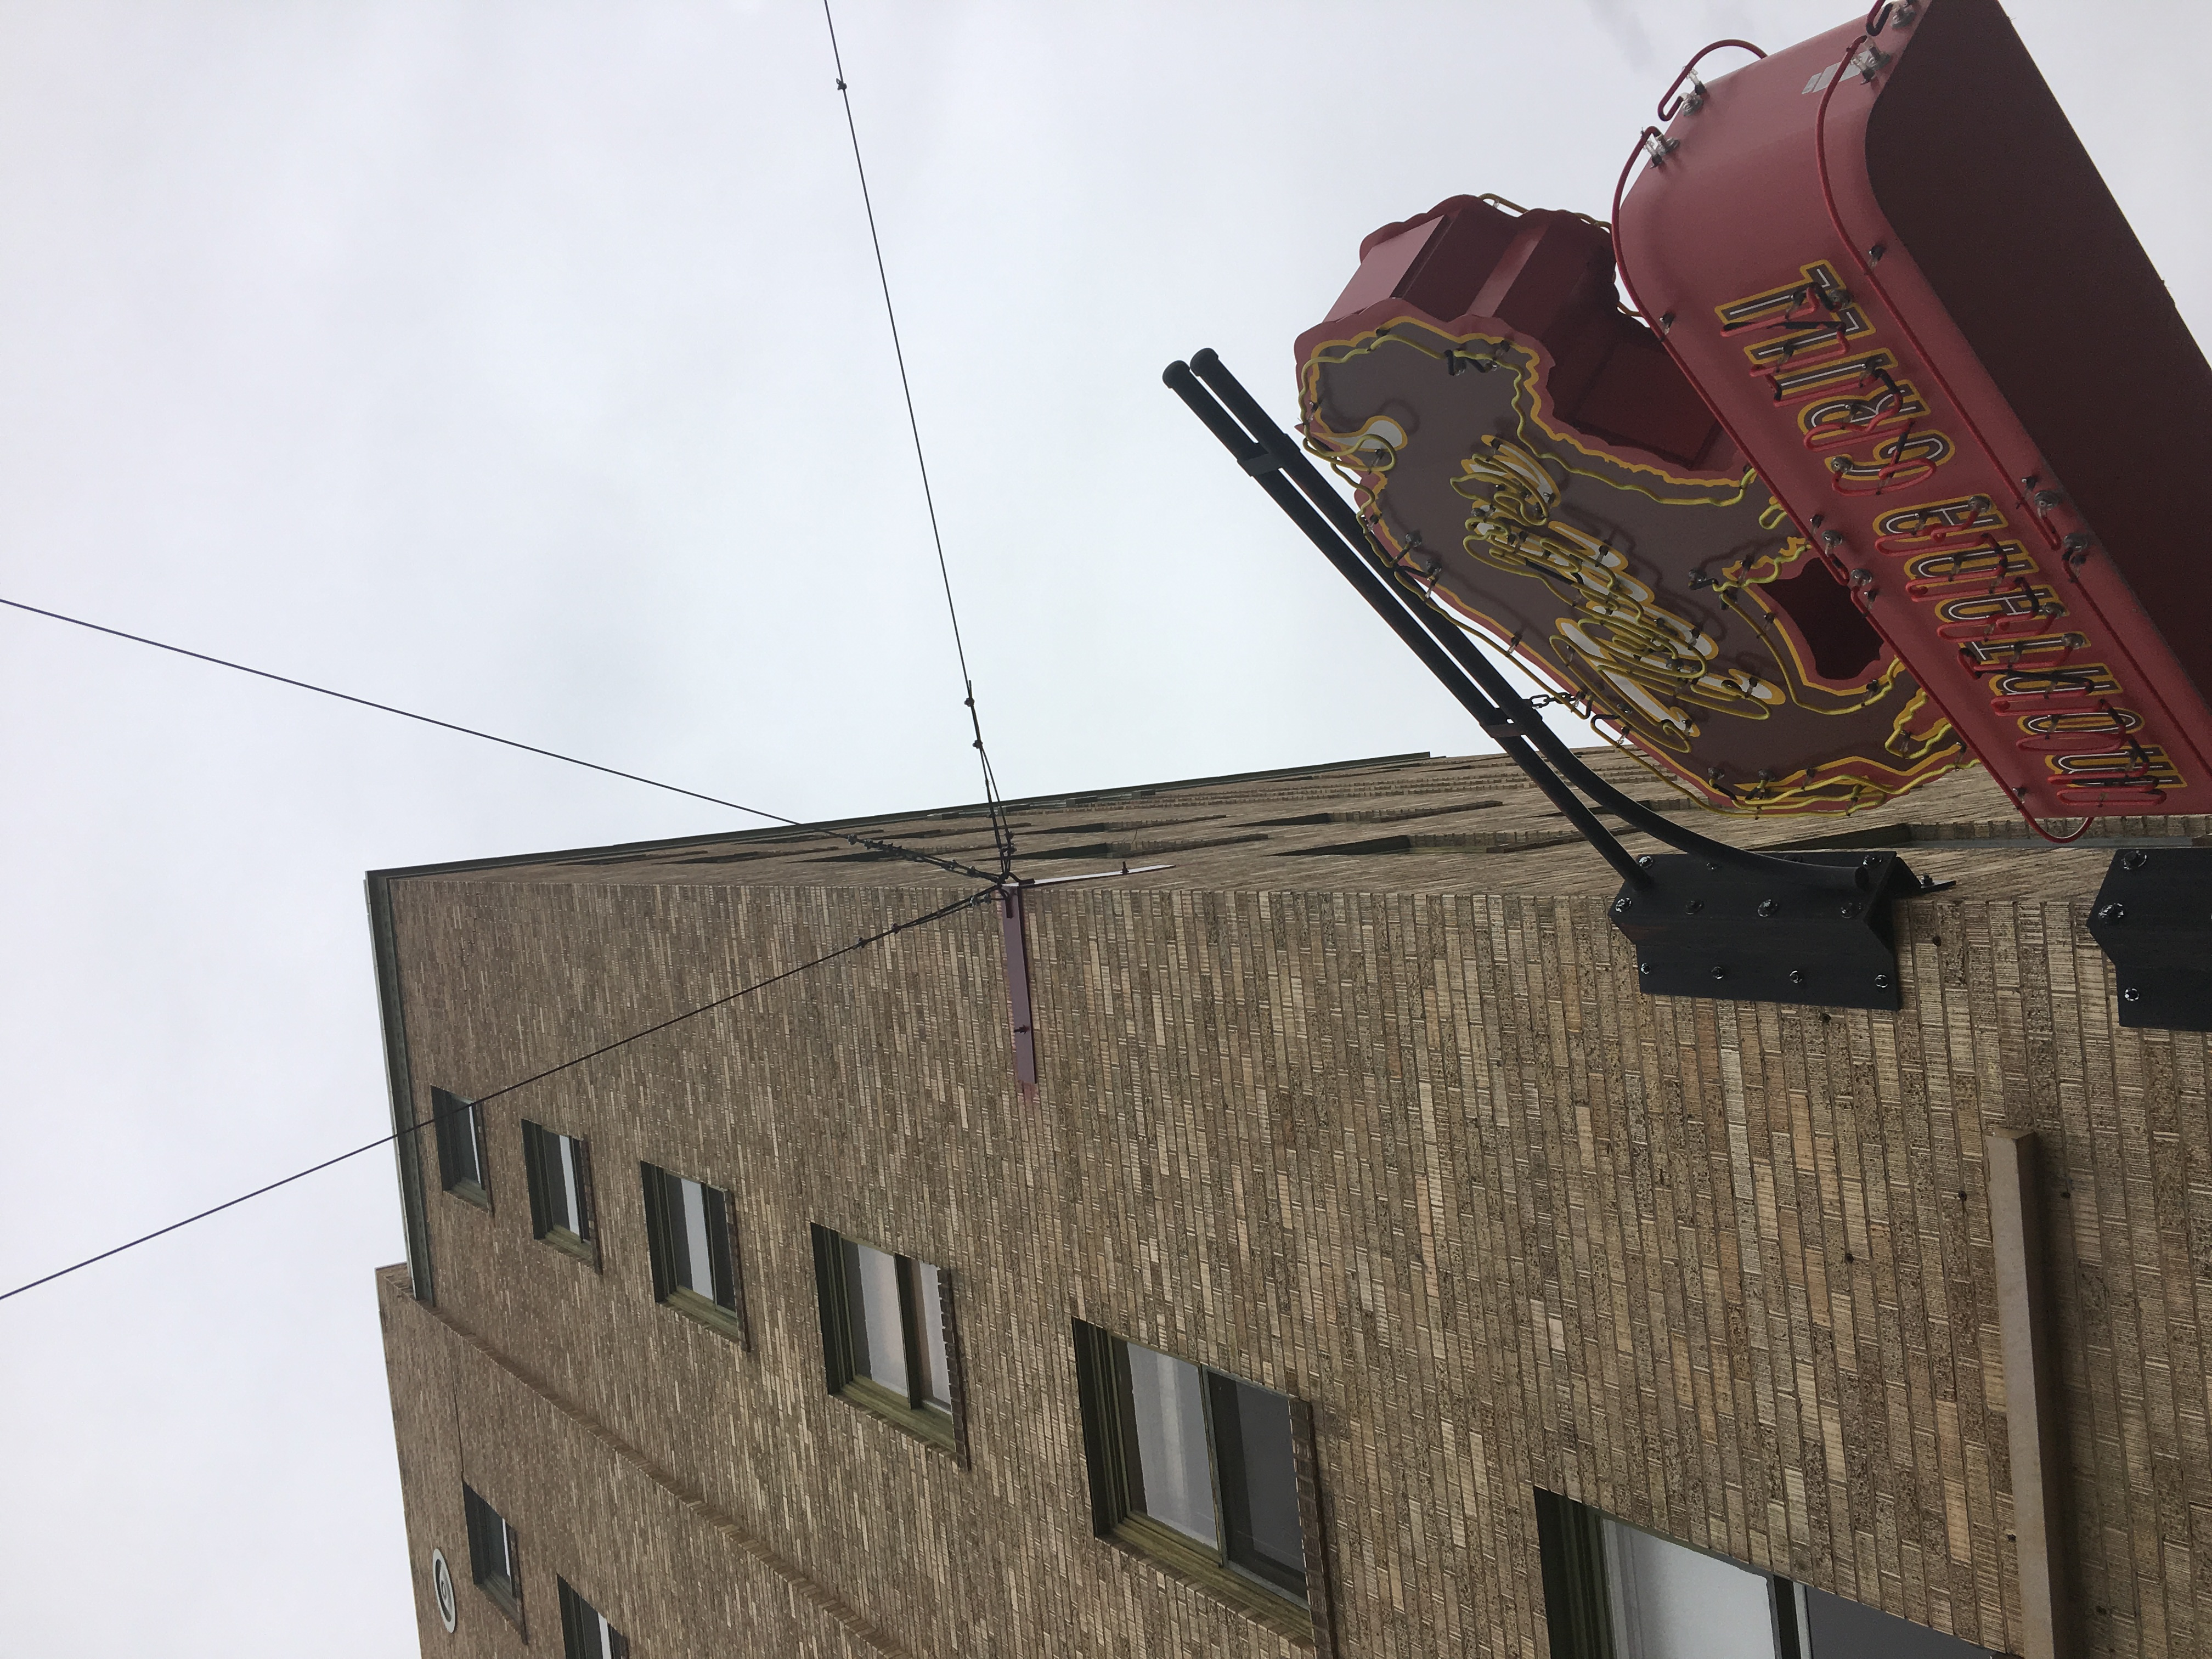
\includegraphics[width=\textwidth]{house4pic1.jpg}
    		\caption{Baxter Hotel}
  		\end{minipage}
  \hfill
  		\begin{minipage}[b]{0.25\textwidth}
    		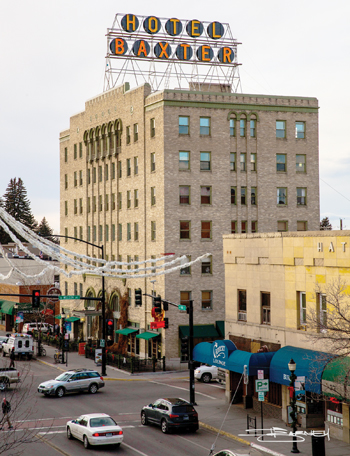
\includegraphics[width=\textwidth]{house4pic2.jpg}
    		\caption{Baxter Hotel}
  		\end{minipage}
\end{figure}

The Baxter Hotel is arguably the most iconic building in Bozeman. Its original opening was in 1929. It was modeled in Art Deco style. Originally the hotel had a total of 76 rooms and two bars. However the interior of the building was under construction until the early 50's. It was remodeled in the 70's and again in the 80's under its new owner. There have been more renovations after that, but they have been rather minor. The Baxter Hotel sign is 32-feet high and 45-feet wide. It was modeled as a beacon to passerbyers.
%%%%%%%%%%%%%%%%%%%%%%%%%%%%%%%%%%%%%%%%%%%%%%%%%%%%%%%%%%%%%
\\
Sources:\\
\\
http://www.searchbozemanareahomes.com/homes/mt/bozeman/gallmtresad217654217654/719-n-wallace-avenue-bozeman-mt-59715
\\\\
http://www.searchbozemanareahomes.com/homes/mt/bozeman/gallmtresad216381216381/725-s-willson-avenue-bozeman-mt-59715
\\\\
http://www.searchbozemanareahomes.com/homes/mt/bozeman/gallmtresad218566218566/711-n-black-bozeman-mt-59715
\\\\
http://www.thebaxterhotel.com/history/
\end{document}